\chapter*{About the Author}
\addcontentsline{toc}{chapter}{About the Author}
\begin{center}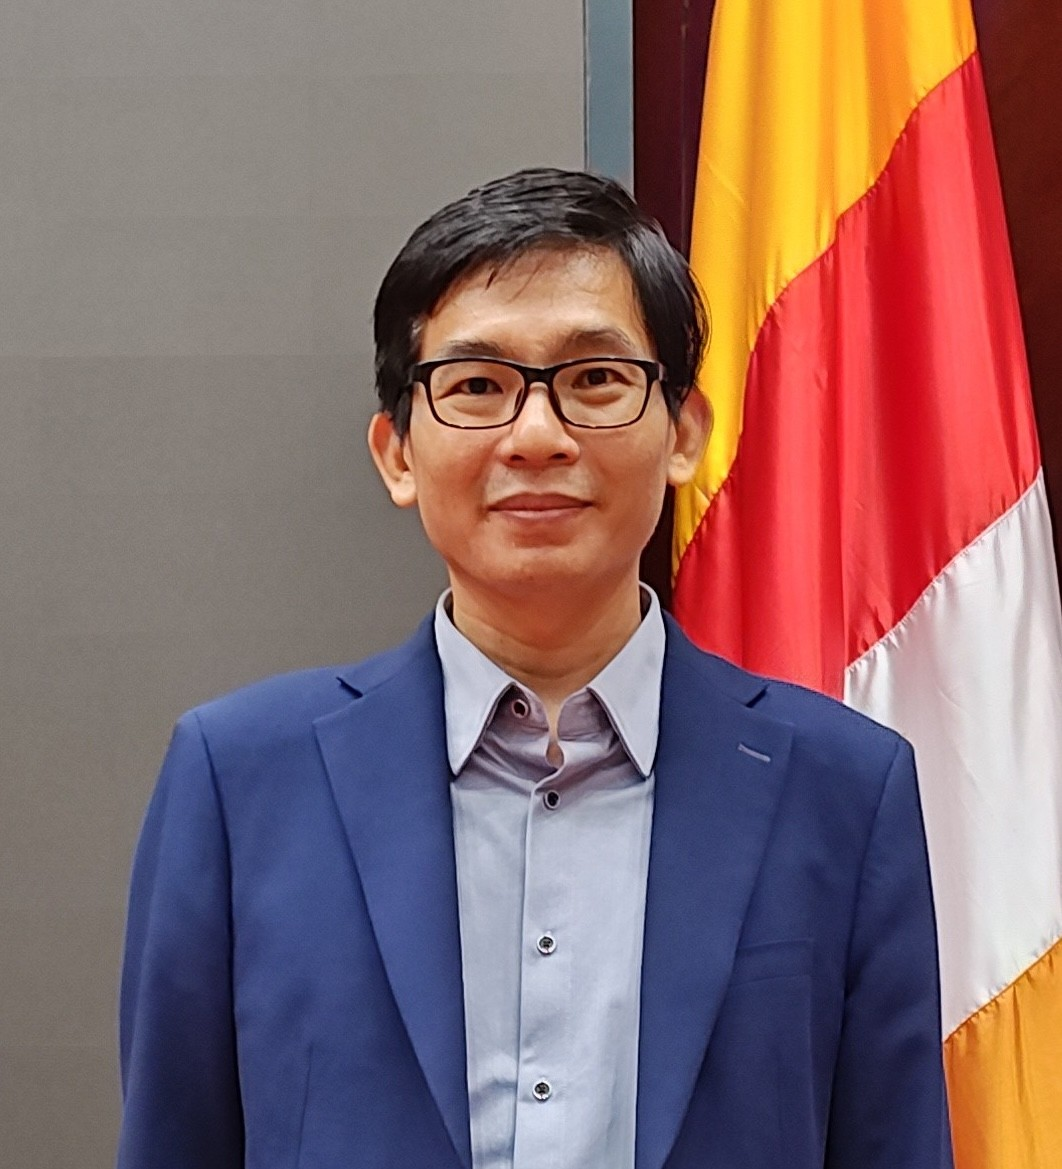
\includegraphics[width=0.38\linewidth]{figures/provided/author.jpg}\end{center}

\textbf{Dr. Rina Buoy} ({\khmerfont ប៊ួយ រីណា}) is an AI researcher, engineer and teacher in Phnom Penh. She holds a PhD in Intelligent Informatics from Osaka Metropolitan University (2024). She is a Senior AI Researcher and Engineer at Techo Startup Center, Ministry of Economy and Finance, where she leads Khmer natural language processing and OCR work behind e-KYC services, and a Visiting Researcher at Osaka Metropolitan University.


Her research focuses on Khmer OCR and NLP, scene text recognition, document layout analysis, machine translation, and large language models and agents. She has published more than 20 peer-reviewed papers, including in IEEE Access, IJDAR and ICDAR, and is Principal Investigator on a JSPS KAKENHI grant on low-resource language document analysis (2026–2029).


Since 2020 she has taught AI, NLP, deep learning, reinforcement learning and computer vision as an adjunct lecturer at several Cambodian universities, and she runs AI training for businesses, professionals and secondary students through \textbf{RinAI}, an academy that trains Cambodians “from non-technical to technical”. Her recognitions include Best Digital R\&D of the Year (Cambodia Digital Awards 2022), a Teaching Excellence award from Paragon International University (2022) and the OxML 2023 Kaggle competition win.


\emph{No-code AI for Young Cambodian Learners} grew out of her \emph{Build Your Own AI} course for Grades 7–12.


\textbf{Learn more:} https://academy.rinabuoy.com

